% Created by tikzDevice version 0.12.3.1 on 2021-06-01 06:57:30
% !TEX encoding = UTF-8 Unicode
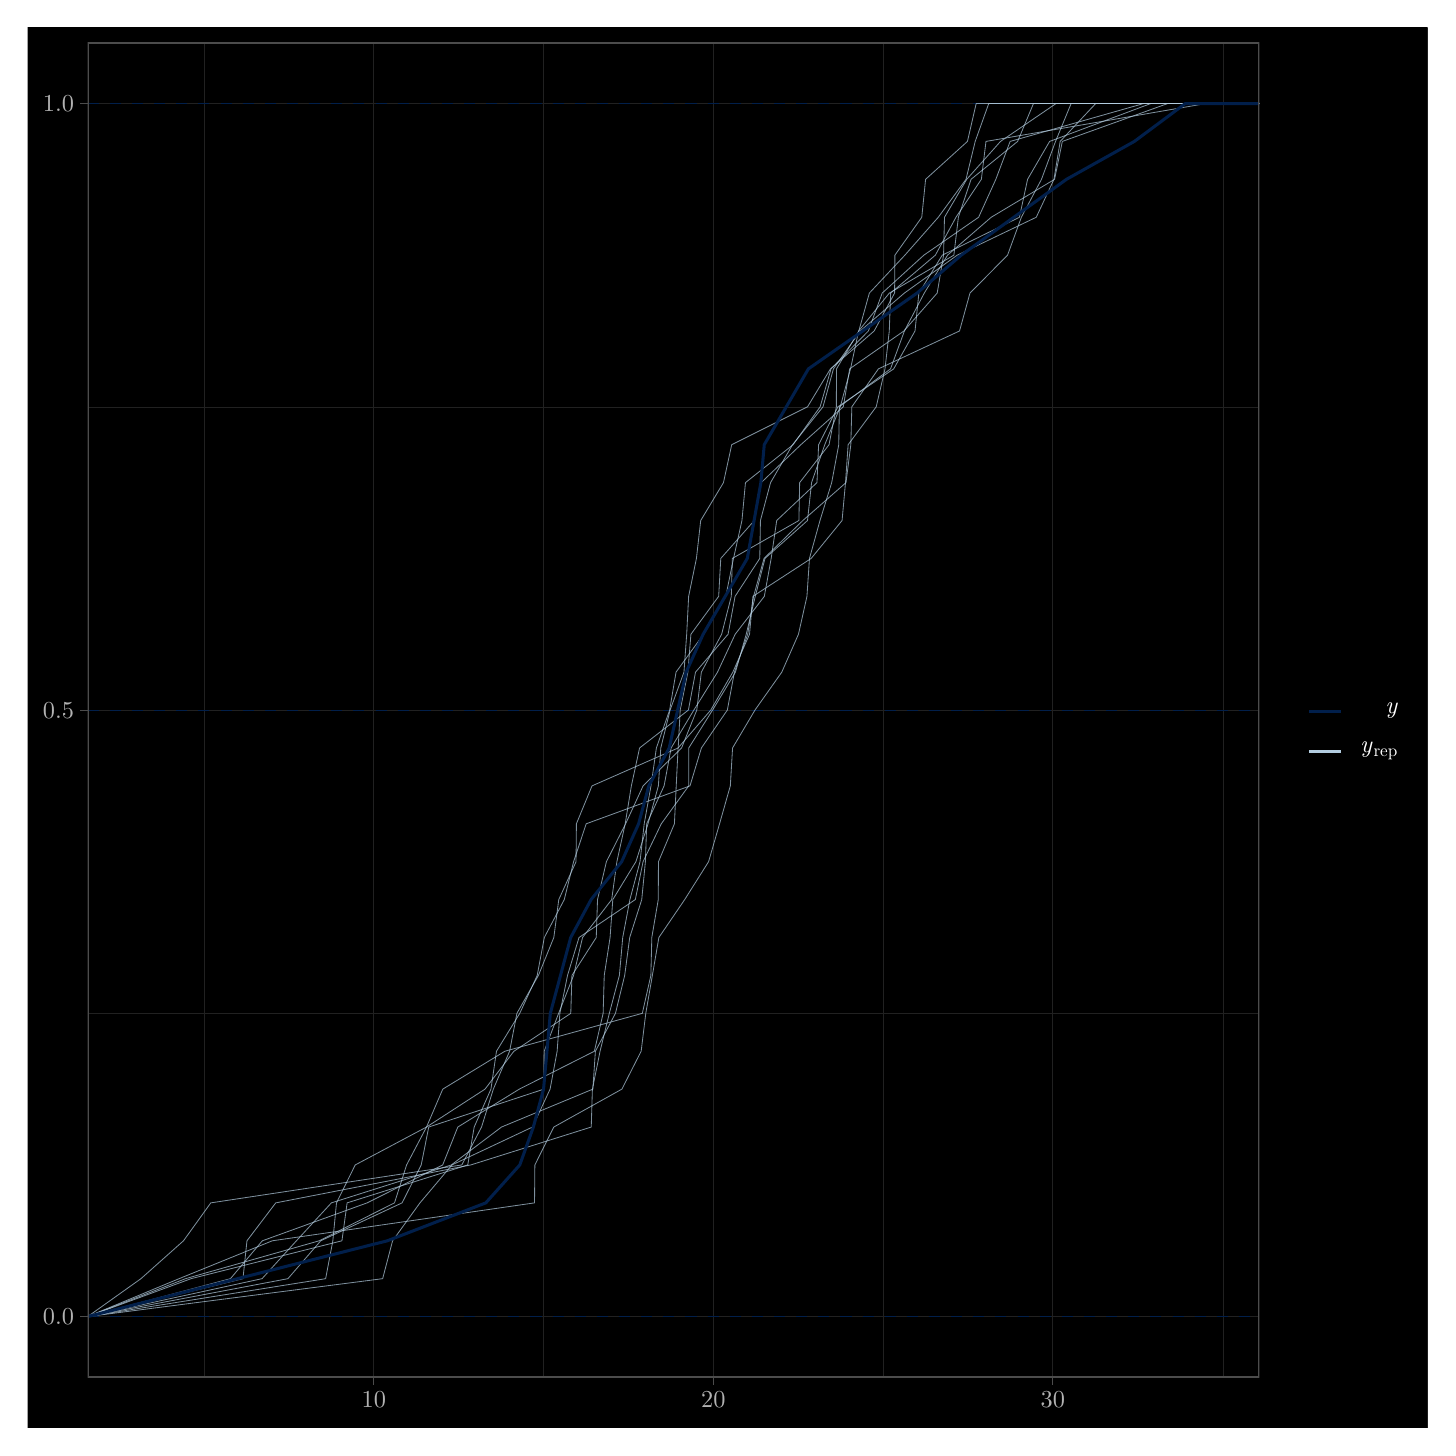
\begin{tikzpicture}[x=1pt,y=1pt]
\definecolor{fillColor}{RGB}{255,255,255}
\path[use as bounding box,fill=fillColor,fill opacity=0.00] (0,0) rectangle (505.89,505.89);
\begin{scope}
\path[clip] (  0.00,  0.00) rectangle (505.89,505.89);
\definecolor{drawColor}{RGB}{0,0,0}
\definecolor{fillColor}{RGB}{0,0,0}

\path[draw=drawColor,line width= 0.6pt,line join=round,line cap=round,fill=fillColor] (  0.00,  0.00) rectangle (505.89,505.89);
\end{scope}
\begin{scope}
\path[clip] ( 21.69, 18.22) rectangle (445.03,500.39);
\definecolor{fillColor}{RGB}{0,0,0}

\path[fill=fillColor] ( 21.69, 18.22) rectangle (445.03,500.39);
\definecolor{drawColor}{gray}{0.13}

\path[draw=drawColor,line width= 0.1pt,line join=round] ( 21.69,149.72) --
	(445.03,149.72);

\path[draw=drawColor,line width= 0.1pt,line join=round] ( 21.69,368.89) --
	(445.03,368.89);

\path[draw=drawColor,line width= 0.1pt,line join=round] ( 63.71, 18.22) --
	( 63.71,500.39);

\path[draw=drawColor,line width= 0.1pt,line join=round] (186.41, 18.22) --
	(186.41,500.39);

\path[draw=drawColor,line width= 0.1pt,line join=round] (309.11, 18.22) --
	(309.11,500.39);

\path[draw=drawColor,line width= 0.1pt,line join=round] (431.81, 18.22) --
	(431.81,500.39);

\path[draw=drawColor,line width= 0.3pt,line join=round] ( 21.69, 40.14) --
	(445.03, 40.14);

\path[draw=drawColor,line width= 0.3pt,line join=round] ( 21.69,259.31) --
	(445.03,259.31);

\path[draw=drawColor,line width= 0.3pt,line join=round] ( 21.69,478.47) --
	(445.03,478.47);

\path[draw=drawColor,line width= 0.3pt,line join=round] (125.06, 18.22) --
	(125.06,500.39);

\path[draw=drawColor,line width= 0.3pt,line join=round] (247.76, 18.22) --
	(247.76,500.39);

\path[draw=drawColor,line width= 0.3pt,line join=round] (370.46, 18.22) --
	(370.46,500.39);
\definecolor{drawColor}{RGB}{1,31,75}

\path[draw=drawColor,line width= 0.1pt,dash pattern=on 4pt off 4pt ,line join=round] ( 21.69,259.31) -- (445.03,259.31);

\path[draw=drawColor,line width= 0.2pt,dash pattern=on 4pt off 4pt ,line join=round] ( 21.69, 40.14) -- (445.03, 40.14);

\path[draw=drawColor,line width= 0.2pt,dash pattern=on 4pt off 4pt ,line join=round] ( 21.69,478.47) -- (445.03,478.47);
\definecolor{drawColor}{RGB}{179,205,224}

\path[draw=drawColor,draw opacity=0.70,line width= 0.3pt,line join=round] ( 21.69, 40.14) --
	( 57.05, 53.84) --
	(105.35, 67.53) --
	(132.55, 81.23) --
	(136.92, 94.93) --
	(144.12,108.63) --
	(149.99,122.33) --
	(172.43,136.02) --
	(222.10,149.72) --
	(225.19,163.42) --
	(225.53,177.12) --
	(227.86,190.82) --
	(227.93,204.51) --
	(233.70,218.21) --
	(234.35,231.91) --
	(235.02,245.61) --
	(246.84,259.31) --
	(254.80,273.00) --
	(260.84,286.70) --
	(262.07,300.40) --
	(283.12,314.10) --
	(294.28,327.80) --
	(295.52,341.49) --
	(296.47,355.19) --
	(306.62,368.89) --
	(309.79,382.59) --
	(311.34,396.29) --
	(311.83,409.98) --
	(327.99,423.68) --
	(335.44,437.38) --
	(344.61,451.08) --
	(346.28,464.78) --
	(425.78,478.47) --
	(445.03,478.47);

\path[draw=drawColor,draw opacity=0.70,line width= 0.3pt,line join=round] ( 21.69, 40.14) --
	( 94.04, 53.84) --
	(105.90, 67.53) --
	(135.29, 81.23) --
	(142.21, 94.93) --
	(144.92,108.63) --
	(186.54,122.33) --
	(186.64,136.02) --
	(191.86,149.72) --
	(197.26,163.42) --
	(200.50,177.12) --
	(211.03,190.82) --
	(212.91,204.51) --
	(215.91,218.21) --
	(218.14,231.91) --
	(221.11,245.61) --
	(238.75,259.31) --
	(241.32,273.00) --
	(253.09,286.70) --
	(255.62,300.40) --
	(264.54,314.10) --
	(264.78,327.80) --
	(268.44,341.49) --
	(276.38,355.19) --
	(287.39,368.89) --
	(291.16,382.59) --
	(300.84,396.29) --
	(316.79,409.98) --
	(335.89,423.68) --
	(364.45,437.38) --
	(370.84,451.08) --
	(373.09,464.78) --
	(385.93,478.47) --
	(445.03,478.47);

\path[draw=drawColor,draw opacity=0.70,line width= 0.3pt,line join=round] ( 21.69, 40.14) --
	( 77.79, 53.84) --
	( 79.24, 67.53) --
	( 89.64, 81.23) --
	(160.09, 94.93) --
	(203.64,108.63) --
	(204.06,122.33) --
	(206.83,136.02) --
	(210.18,149.72) --
	(213.81,163.42) --
	(215.02,177.12) --
	(217.61,190.82) --
	(221.27,204.51) --
	(222.78,218.21) --
	(225.23,231.91) --
	(227.18,245.61) --
	(231.97,259.31) --
	(234.28,273.00) --
	(244.22,286.70) --
	(252.26,300.40) --
	(255.06,314.10) --
	(258.10,327.80) --
	(259.37,341.49) --
	(276.57,355.19) --
	(286.36,368.89) --
	(290.29,382.59) --
	(303.79,396.29) --
	(308.78,409.98) --
	(323.83,423.68) --
	(343.62,437.38) --
	(349.84,451.08) --
	(355.00,464.78) --
	(403.27,478.47) --
	(445.03,478.47);

\path[draw=drawColor,draw opacity=0.70,line width= 0.3pt,line join=round] ( 21.69, 40.14) --
	( 40.93, 53.84) --
	( 56.31, 67.53) --
	( 66.17, 81.23) --
	(156.87, 94.93) --
	(164.00,108.63) --
	(168.26,122.33) --
	(174.14,136.02) --
	(176.79,149.72) --
	(184.56,163.42) --
	(190.12,177.12) --
	(191.91,190.82) --
	(198.15,204.51) --
	(198.28,218.21) --
	(203.92,231.91) --
	(235.06,245.61) --
	(235.79,259.31) --
	(238.56,273.00) --
	(239.66,286.70) --
	(249.69,300.40) --
	(250.45,314.10) --
	(262.57,327.80) --
	(265.04,341.49) --
	(279.38,355.19) --
	(294.72,368.89) --
	(297.02,382.59) --
	(316.63,396.29) --
	(328.65,409.98) --
	(330.95,423.68) --
	(331.29,437.38) --
	(339.32,451.08) --
	(351.53,464.78) --
	(371.60,478.47) --
	(445.03,478.47);

\path[draw=drawColor,draw opacity=0.70,line width= 0.3pt,line join=round] ( 21.69, 40.14) --
	(107.67, 53.84) --
	(110.27, 67.53) --
	(111.59, 81.23) --
	(118.35, 94.93) --
	(144.12,108.63) --
	(165.26,122.33) --
	(175.69,136.02) --
	(196.25,149.72) --
	(196.67,163.42) --
	(205.45,177.12) --
	(205.91,190.82) --
	(209.12,204.51) --
	(216.06,218.21) --
	(222.38,231.91) --
	(236.29,245.61) --
	(241.78,259.31) --
	(243.43,273.00) --
	(250.76,286.70) --
	(254.25,300.40) --
	(254.63,314.10) --
	(278.68,327.80) --
	(278.95,341.49) --
	(289.57,355.19) --
	(292.21,368.89) --
	(292.27,382.59) --
	(300.33,396.29) --
	(304.14,409.98) --
	(316.97,423.68) --
	(329.05,437.38) --
	(339.06,451.08) --
	(342.38,464.78) --
	(347.28,478.47) --
	(445.03,478.47);

\path[draw=drawColor,draw opacity=0.70,line width= 0.3pt,line join=round] ( 21.69, 40.14) --
	( 54.72, 53.84) --
	( 88.40, 67.53) --
	(183.15, 81.23) --
	(183.27, 94.93) --
	(190.11,108.63) --
	(214.72,122.33) --
	(221.68,136.02) --
	(223.35,149.72) --
	(225.73,163.42) --
	(228.08,177.12) --
	(237.41,190.82) --
	(246.04,204.51) --
	(250.01,218.21) --
	(253.90,231.91) --
	(254.71,245.61) --
	(262.81,259.31) --
	(272.49,273.00) --
	(278.52,286.70) --
	(281.59,300.40) --
	(282.50,314.10) --
	(286.30,327.80) --
	(290.53,341.49) --
	(293.08,355.19) --
	(293.30,368.89) --
	(311.79,382.59) --
	(316.81,396.29) --
	(323.98,409.98) --
	(332.39,423.68) --
	(348.17,437.38) --
	(371.06,451.08) --
	(373.87,464.78) --
	(411.95,478.47) --
	(445.03,478.47);

\path[draw=drawColor,draw opacity=0.70,line width= 0.3pt,line join=round] ( 21.69, 40.14) --
	( 59.04, 53.84) --
	(113.56, 67.53) --
	(115.43, 81.23) --
	(159.02, 94.93) --
	(161.34,108.63) --
	(167.40,122.33) --
	(169.40,136.02) --
	(177.81,149.72) --
	(184.12,163.42) --
	(186.69,177.12) --
	(193.90,190.82) --
	(197.27,204.51) --
	(201.82,218.21) --
	(239.32,231.91) --
	(243.45,245.61) --
	(252.82,259.31) --
	(255.38,273.00) --
	(260.19,286.70) --
	(262.31,300.40) --
	(266.08,314.10) --
	(280.11,327.80) --
	(295.70,341.49) --
	(297.44,355.19) --
	(297.81,368.89) --
	(307.41,382.59) --
	(336.72,396.29) --
	(340.50,409.98) --
	(354.07,423.68) --
	(359.07,437.38) --
	(366.33,451.08) --
	(371.41,464.78) --
	(377.05,478.47) --
	(445.03,478.47);

\path[draw=drawColor,draw opacity=0.70,line width= 0.3pt,line join=round] ( 21.69, 40.14) --
	( 73.27, 53.84) --
	( 84.80, 67.53) --
	(122.67, 81.23) --
	(149.97, 94.93) --
	(155.43,108.63) --
	(177.65,122.33) --
	(204.77,136.02) --
	(207.94,149.72) --
	(208.34,163.42) --
	(210.45,177.12) --
	(211.43,190.82) --
	(219.78,204.51) --
	(224.16,218.21) --
	(227.90,231.91) --
	(228.77,245.61) --
	(232.14,259.31) --
	(237.15,273.00) --
	(238.13,286.70) --
	(238.84,300.40) --
	(241.65,314.10) --
	(243.20,327.80) --
	(251.42,341.49) --
	(254.40,355.19) --
	(281.80,368.89) --
	(290.08,382.59) --
	(305.88,396.29) --
	(313.26,409.98) --
	(313.37,423.68) --
	(323.08,437.38) --
	(324.46,451.08) --
	(339.58,464.78) --
	(342.74,478.47) --
	(445.03,478.47);

\path[draw=drawColor,draw opacity=0.70,line width= 0.3pt,line join=round] ( 21.69, 40.14) --
	(128.27, 53.84) --
	(131.86, 67.53) --
	(141.75, 81.23) --
	(153.31, 94.93) --
	(182.41,108.63) --
	(188.77,122.33) --
	(191.32,136.02) --
	(192.31,149.72) --
	(195.07,163.42) --
	(199.23,177.12) --
	(219.57,190.82) --
	(222.37,204.51) --
	(228.95,218.21) --
	(238.87,231.91) --
	(238.88,245.61) --
	(247.49,259.31) --
	(255.75,273.00) --
	(259.65,286.70) --
	(262.91,300.40) --
	(266.43,314.10) --
	(281.79,327.80) --
	(283.26,341.49) --
	(288.03,355.19) --
	(293.62,368.89) --
	(297.33,382.59) --
	(300.27,396.29) --
	(311.36,409.98) --
	(334.67,423.68) --
	(336.31,437.38) --
	(340.88,451.08) --
	(357.72,464.78) --
	(363.44,478.47) --
	(445.03,478.47);

\path[draw=drawColor,draw opacity=0.70,line width= 0.3pt,line join=round] ( 21.69, 40.14) --
	( 84.69, 53.84) --
	( 97.11, 67.53) --
	(109.75, 81.23) --
	(153.08, 94.93) --
	(171.21,108.63) --
	(204.23,122.33) --
	(205.14,136.02) --
	(212.39,149.72) --
	(215.73,163.42) --
	(217.54,177.12) --
	(221.89,190.82) --
	(223.21,204.51) --
	(223.68,218.21) --
	(229.97,231.91) --
	(232.51,245.61) --
	(240.73,259.31) --
	(249.27,273.00) --
	(255.65,286.70) --
	(266.19,300.40) --
	(268.66,314.10) --
	(270.66,327.80) --
	(285.21,341.49) --
	(285.80,355.19) --
	(292.78,368.89) --
	(312.93,382.59) --
	(320.64,396.29) --
	(322.03,409.98) --
	(330.48,423.68) --
	(358.37,437.38) --
	(361.31,451.08) --
	(369.27,464.78) --
	(405.84,478.47) --
	(445.03,478.47);
\definecolor{drawColor}{RGB}{1,31,75}

\path[draw=drawColor,line width= 1.1pt,line join=round] ( 21.69, 40.14) --
	(129.97, 67.53) --
	(165.55, 81.23) --
	(177.82, 94.93) --
	(182.73,108.63) --
	(186.41,122.33) --
	(188.86,149.72) --
	(192.54,163.42) --
	(196.22,177.12) --
	(203.59,190.82) --
	(214.63,204.51) --
	(220.76,218.21) --
	(224.44,231.91) --
	(231.81,245.61) --
	(237.94,273.00) --
	(244.08,286.70) --
	(260.03,314.10) --
	(264.94,341.49) --
	(266.16,355.19) --
	(282.11,382.59) --
	(301.75,396.29) --
	(321.38,409.98) --
	(337.33,423.68) --
	(375.36,451.08) --
	(399.90,464.78) --
	(418.31,478.47) --
	(445.03,478.47);
\definecolor{drawColor}{RGB}{76,76,76}

\path[draw=drawColor,line width= 0.6pt,line join=round,line cap=round] ( 21.69, 18.22) rectangle (445.03,500.39);
\end{scope}
\begin{scope}
\path[clip] (  0.00,  0.00) rectangle (505.89,505.89);
\definecolor{drawColor}{RGB}{178,178,178}

\node[text=drawColor,anchor=base east,inner sep=0pt, outer sep=0pt, scale=  0.88] at ( 16.74, 37.11) {0.0};

\node[text=drawColor,anchor=base east,inner sep=0pt, outer sep=0pt, scale=  0.88] at ( 16.74,256.28) {0.5};

\node[text=drawColor,anchor=base east,inner sep=0pt, outer sep=0pt, scale=  0.88] at ( 16.74,475.44) {1.0};
\end{scope}
\begin{scope}
\path[clip] (  0.00,  0.00) rectangle (505.89,505.89);
\definecolor{drawColor}{RGB}{76,76,76}

\path[draw=drawColor,line width= 0.3pt,line join=round] ( 18.94, 40.14) --
	( 21.69, 40.14);

\path[draw=drawColor,line width= 0.3pt,line join=round] ( 18.94,259.31) --
	( 21.69,259.31);

\path[draw=drawColor,line width= 0.3pt,line join=round] ( 18.94,478.47) --
	( 21.69,478.47);
\end{scope}
\begin{scope}
\path[clip] (  0.00,  0.00) rectangle (505.89,505.89);
\definecolor{drawColor}{RGB}{76,76,76}

\path[draw=drawColor,line width= 0.3pt,line join=round] (125.06, 15.47) --
	(125.06, 18.22);

\path[draw=drawColor,line width= 0.3pt,line join=round] (247.76, 15.47) --
	(247.76, 18.22);

\path[draw=drawColor,line width= 0.3pt,line join=round] (370.46, 15.47) --
	(370.46, 18.22);
\end{scope}
\begin{scope}
\path[clip] (  0.00,  0.00) rectangle (505.89,505.89);
\definecolor{drawColor}{RGB}{178,178,178}

\node[text=drawColor,anchor=base,inner sep=0pt, outer sep=0pt, scale=  0.88] at (125.06,  7.21) {10};

\node[text=drawColor,anchor=base,inner sep=0pt, outer sep=0pt, scale=  0.88] at (247.76,  7.21) {20};

\node[text=drawColor,anchor=base,inner sep=0pt, outer sep=0pt, scale=  0.88] at (370.46,  7.21) {30};
\end{scope}
\begin{scope}
\path[clip] (  0.00,  0.00) rectangle (505.89,505.89);
\definecolor{fillColor}{RGB}{0,0,0}

\path[fill=fillColor] (456.03,231.74) rectangle (500.39,286.87);
\end{scope}
\begin{scope}
\path[clip] (  0.00,  0.00) rectangle (505.89,505.89);
\definecolor{fillColor}{RGB}{0,0,0}

\path[fill=fillColor] (461.53,251.70) rectangle (475.98,266.15);
\end{scope}
\begin{scope}
\path[clip] (  0.00,  0.00) rectangle (505.89,505.89);
\definecolor{drawColor}{RGB}{1,31,75}

\path[draw=drawColor,draw opacity=0.70,line width= 0.3pt,line join=round] (462.97,258.93) -- (474.53,258.93);
\end{scope}
\begin{scope}
\path[clip] (  0.00,  0.00) rectangle (505.89,505.89);
\definecolor{drawColor}{RGB}{1,31,75}

\path[draw=drawColor,line width= 1.1pt,line join=round] (462.97,258.93) -- (474.53,258.93);
\end{scope}
\begin{scope}
\path[clip] (  0.00,  0.00) rectangle (505.89,505.89);
\definecolor{fillColor}{RGB}{0,0,0}

\path[fill=fillColor] (461.53,237.24) rectangle (475.98,251.70);
\end{scope}
\begin{scope}
\path[clip] (  0.00,  0.00) rectangle (505.89,505.89);
\definecolor{drawColor}{RGB}{179,205,224}

\path[draw=drawColor,draw opacity=0.70,line width= 0.3pt,line join=round] (462.97,244.47) -- (474.53,244.47);
\end{scope}
\begin{scope}
\path[clip] (  0.00,  0.00) rectangle (505.89,505.89);
\definecolor{drawColor}{RGB}{179,205,224}

\path[draw=drawColor,line width= 1.1pt,line join=round] (462.97,244.47) -- (474.53,244.47);
\end{scope}
\begin{scope}
\path[clip] (  0.00,  0.00) rectangle (505.89,505.89);
\definecolor{drawColor}{RGB}{255,255,255}

\node[text=drawColor,anchor=base west,inner sep=0pt, outer sep=0pt, scale=  0.88] at (490.62,257.89) {\itshape y};
\end{scope}
\begin{scope}
\path[clip] (  0.00,  0.00) rectangle (505.89,505.89);
\definecolor{drawColor}{RGB}{255,255,255}

\node[text=drawColor,anchor=base west,inner sep=0pt, outer sep=0pt, scale=  0.88] at (481.48,243.84) {\itshape y};

\node[text=drawColor,anchor=base west,inner sep=0pt, outer sep=0pt, scale=  0.62] at (486.32,242.51) {r};

\node[text=drawColor,anchor=base west,inner sep=0pt, outer sep=0pt, scale=  0.62] at (488.73,242.51) {e};

\node[text=drawColor,anchor=base west,inner sep=0pt, outer sep=0pt, scale=  0.62] at (491.47,242.51) {p};
\end{scope}
\end{tikzpicture}
